
% xetex expected
\documentclass[xetex,professionalfont]{beamer}

% we want math
\usepackage{amsmath}

% fixes and extensions to amsmath
\usepackage{mathtools}

% additional math symbols
\usepackage{amssymb}

% good-looking fractions in text via \sfrac
\usepackage{xfrac}

% fix spaces after custom commands (see below for examples)
\usepackage{xspace}

% minted allows for fancy syntax highlighting (requires python with pygments)
% usage:
%   \begin{minted}{python}
%   codeb
%   \end{minted}
% \usepackage{minted}

% better looking tables
% usage:
%   begin with a \toprule, write a single row of column headings,
%   then add \midrule and after the columns of data we finish with \bottomrule
% example:
%   \begin{tabular}{llr} \toprule
%   Animal & Description & Price \midrule
%   cat & foo & 10 \\
%   dog & bar & 20 \\ \bottomrule
%   \end{tabular}
% note that good tables generally neither have vertical rules nor double rules
\usepackage{booktabs}

% system font support (requires xetex or luatex)
\usepackage{fontspec}
\setmonofont[Scale=0.7]{Cousine} % part of ttf-chromeos fonts on Arch

% multi-language quotes for babel
\usepackage{csquotes}

% easy way to include copyright information
\usepackage{copyrightbox}

% better bibliographies
\usepackage[backend=biber,style=authoryear]{biblatex}

% language support (english,ngerman)
\usepackage[english]{babel}

% -----------------------------------------------------------------------------

% specify PDF metadata
\hypersetup{pdftitle={CVSP UE - Preview},pdfsubject={},pdfauthor={Christopher Pramerdorfer}}

% copyright font style
\makeatletter\renewcommand{\CRB@setcopyrightfont}{\tiny\color{lightgray}}

% add bib file
\addbibresource{literature.bib}

% use tuwcvl beamer theme
\usetheme{tuwcvl}

% -----------------------------------------------------------------------------

% common english abbreviations
\newcommand{\ie}{\mbox{i.e.}\xspace} % i.e.
\newcommand{\eg}{\mbox{e.g.}\xspace} % e.g.

% math - argmin and argmax
\DeclareMathOperator*{\argmin}{arg\,min}
\DeclareMathOperator*{\argmax}{arg\,max}

% shortcuts for number ranges
\newcommand{\NN}{\mathbb{N}}
\newcommand{\ZZ}{\mathbb{Z}}
\newcommand{\QQ}{\mathbb{Q}}
\newcommand{\RR}{\mathbb{R}}

% bold vectors
\renewcommand{\vec}[1]{\ensuremath{\mathbf{#1}}}

% vector shortcuts
\newcommand{\va}{\vec{a}}
\newcommand{\vb}{\vec{b}}
\newcommand{\vc}{\vec{c}}
\newcommand{\ve}{\vec{e}}
\newcommand{\vr}{\vec{r}}
\newcommand{\vs}{\vec{s}}
\newcommand{\vt}{\vec{t}}
\newcommand{\vu}{\vec{u}}
\newcommand{\vv}{\vec{v}}
\newcommand{\vw}{\vec{w}}
\newcommand{\vx}{\vec{x}}
\newcommand{\vy}{\vec{y}}
\newcommand{\vz}{\vec{z}}

% highlight
\newcommand{\highlight}[1]{\textcolor{tuwcvl_inf_red}{\textbf{#1}}}

% -----------------------------------------------------------------------------

\title{Computer Vision Systems Programming UE}
\subtitle{Introduction}
\author{Martin Kampel, Christopher Pramerdorfer}
\institute{Computer Vision Lab, Vienna University of Technology}

\begin{document}

% -----------------------------------------------------------------------------

\begin{frame}
\maketitle
\end{frame}

% -----------------------------------------------------------------------------

\begin{frame}
\frametitle{Course Aim}

Improve your skills in applied Computer Vision (CV)
\begin{itemize}
	\item Plan, implement, and test a small CV project
	\item Present it orally and in written form
\end{itemize}

\bigskip
This allows you to
\begin{itemize}
	\item Explore a CV topic of your choice
	\item Apply what you learned in the lecture
	\item Improve your CV programming skills
	\item Practice dissemination
\end{itemize}

\end{frame}

% -----------------------------------------------------------------------------

\begin{frame}
\frametitle{Your Task}

Realize a CV project of your choice
\begin{itemize}
	\item In any programming language you like
	\item Using any \emph{publicly available} libraries you want
	\item As long as the required effort is appropriate
\end{itemize}

\bigskip
Matlab, Python, or C++ recommended
\begin{itemize}
	\item Don't know C++ yet? Now is a good time!
\end{itemize}

\end{frame}

% -----------------------------------------------------------------------------

\begin{frame}
\frametitle{Project Topics}

Choose any CV topic you want, as long as you learn something
\begin{itemize}
	\item Choose something that is new and interesting to you
	\item Finalize topic and scope together with lecturers
\end{itemize}

\end{frame}

% -----------------------------------------------------------------------------

\begin{frame}
\frametitle{Project Topics}
\framesubtitle{Available Sensor Hardware}

Available sensors
\begin{itemize}
	\item Kinect depth sensors
	\item IP camera network with overlapping views (stationary)
	\item Thermal imaging camera (stationary)
	\item Android tablets and phones with cameras
\end{itemize}

\bigskip
Or use existing datasets, your own camera, smartphone, ...

\end{frame}

% -----------------------------------------------------------------------------

\begin{frame}
\frametitle{Project Topics}
\framesubtitle{Proposal -- Balloon Tracking}

Detect and track the balloon in 3D

\bigskip
\begin{center}
	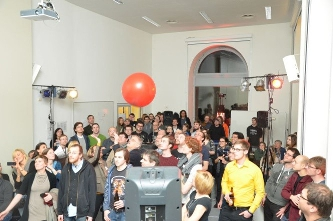
\includegraphics[width=7cm]{figures/balloon.jpg}
\end{center}

\end{frame}

% -----------------------------------------------------------------------------

\begin{frame}
\frametitle{Project Topics}
\framesubtitle{Proposal -- Object Detection in Satellite Images}

Detect streets and certain objects in satellite images

\bigskip
\begin{center}
	\copyrightbox[b]
	{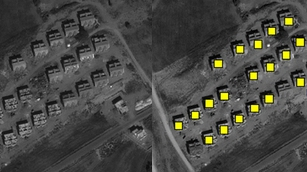
\includegraphics[width=7cm]{figures/satellite-objects.jpg}}
	{\centering Image from \cite{sirmacek2009}}
\end{center}

\end{frame}

% -----------------------------------------------------------------------------

\begin{frame}
\frametitle{Project Topics}
\framesubtitle{Proposal -- Moth Classification}

Distinguish between moth species

\bigskip
\begin{center}
	\copyrightbox[b]
	{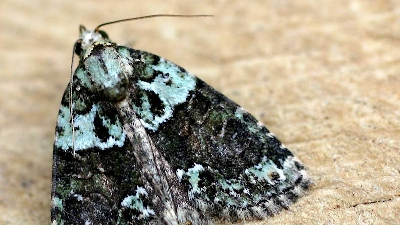
\includegraphics[width=7cm]{figures/moth.jpg}}
	{\centering Image from \url{wikipedia.org}}
\end{center}

\end{frame}

% -----------------------------------------------------------------------------

\begin{frame}
\frametitle{Project Topics}
\framesubtitle{Proposal -- Match Traces Left by Burglars}

Match traces left by burglary tools for forensics

\bigskip
\begin{center}
	
\includegraphics[width=7cm]{figures/burglary-trace.jpg}
\end{center}

\end{frame}

% -----------------------------------------------------------------------------

\begin{frame}
\frametitle{Project Topics}
\framesubtitle{More Proposals}

For more topics and details see \url{http://www.caa.tuwien.ac.at/cvl/bachelorarbeiten-praktika-masterarbeiten/}

\end{frame}

% -----------------------------------------------------------------------------

\begin{frame}
\frametitle{Project Topics}
\framesubtitle{Wurstify: Example Project From Last Year}

Face detection and pose estimation to map beards on faces

\bigskip
\begin{center}
	\copyrightbox[b]
	{
\includegraphics[width=4cm]{figures/wurstify.png}}
	{\centering Image from \url{wurstify.me}}
\end{center}

\end{frame}

% -----------------------------------------------------------------------------

\begin{frame}
\frametitle{Syllabus}

1.\ Select a CV topic according to your interests \highlight{[21.10.]}

\medskip
2.\ Give a short presentation on your project \highlight{[28.10.]}

\medskip
3.\ Implement and test your application \highlight{[17.01.]}

\medskip
4.\ Give a midterm presentation \highlight{[9.12.]}

\medskip
5.\ Write a short report \highlight{[17.01.]}

\medskip
6.\ Give a final presentation \highlight{[20.01.]}

\end{frame}

% -----------------------------------------------------------------------------

\begin{frame}
\frametitle{Syllabus}
\framesubtitle{Topic Selection}

Send a short project proposal to lecturers (\url{cvsp@caa.tuwien.ac.at})

\bigskip
Contents
\begin{itemize}
	\item Name, Matrikelnummer, Studienkennzahl
	\item General introduction to your topic
	\item Definition of the project scope (what are you going to do?)
	\item Languages and libraries you plan to use
\end{itemize}

\bigskip
\highlight{Deadline: 21.10.}

\end{frame}

% -----------------------------------------------------------------------------

\begin{frame}
\frametitle{Syllabus}
\framesubtitle{Initial Presentation}

Give an introduction to your project\\\medskip
Tell us about your project (as in written proposal)\\\medskip
Keep it short (around 5 minutes)

\bigskip
\highlight{28.10., 10:15} at SR 183/2 (here)

\end{frame}

% -----------------------------------------------------------------------------

\begin{frame}
\frametitle{Syllabus}
\framesubtitle{Midterm Presentation}

Briefly recap your project\\\medskip
Focus on progress and current project status\\\medskip
Presentation should take 5 to 10 minutes\\\medskip
Include images and videos of your application

\bigskip
\highlight{9.12., 10:15} at SR 183/2 (here)

\end{frame}

% -----------------------------------------------------------------------------

\begin{frame}
\frametitle{Syllabus}
\framesubtitle{Project Report}

5 to 10 pages long, must include
\begin{itemize} 
	\item A brief explanation of your topic
	\item Scope of your project (what was planned, what changed?)
	\item How you implemented it (language, libraries)
	\item Problems you faced during development
	\item Tests and results
\end{itemize}

\bigskip
Hand in report and project code by email \highlight{until 17.01.}

\end{frame}

% -----------------------------------------------------------------------------

\begin{frame}
\frametitle{Syllabus}
\framesubtitle{Final Presentation}

Cover all topics in your report (see above list)\\\medskip
Presentation should take 10 to 15 minutes\\\medskip
Show a demo of your project (live or video)

\bigskip
\highlight{20.01., 10:15} at SR 183/2 (here)

\end{frame}

% -----------------------------------------------------------------------------

\begin{frame}
\frametitle{Grading}

Initial presentation: 5\% \\\medskip
Midterm presentation: 5\% \\\medskip
Implementation and report: 80\% \\\medskip
Final presentation: 10\%

\bigskip
\highlight{Presentations are mandatory}
\begin{itemize}
	\item Contact us beforehand if you cannot come
\end{itemize}

\end{frame}

% -----------------------------------------------------------------------------

\begin{frame}
\frametitle{Course Assistance}

Assistance mainly via mail (\url{cvsp@caa.tuwien.ac.at})

\bigskip
Weekly timeslot for personal support
\begin{itemize}
	\item On appointment (\url{cvsp@caa.tuwien.ac.at})
	\item Wed 11:45 -- 12:30 (after lecture)
	\item Room HA04-10 (\url{http://www.caa.tuwien.ac.at/cvl/contact/})
\end{itemize}

\bigskip
We expect to stay in touch with you throughout the semester
\begin{itemize}
	\item Contact us if you have questions, problems
\end{itemize}

\bigskip
Follow \texttt{@tuwcvsp} on Twitter for updates

\end{frame}

% -----------------------------------------------------------------------------

\begin{frame}
\frametitle{Prerequisites}

Ability to work independently, manage a small project\\\medskip
Basic image processing and computer vision knowledge\\\medskip
You must be able to develop software on your own
\begin{itemize}
	\item This is \emph{not} a general programming course
\end{itemize}

\end{frame}

% -----------------------------------------------------------------------------

\begin{frame}
\frametitle{Associated Lecture}

We recommend the associated lecture for
\begin{itemize}
	\item CV software and resources
	\item Tips for approaching CV problems
	\item A showcase of interesting CV applications
\end{itemize}

\end{frame}

% -----------------------------------------------------------------------------

\begin{frame}
\frametitle{Bibliography}

\printbibliography

\end{frame}

\end{document}
